\documentclass[conference]{IEEEtran}
\IEEEoverridecommandlockouts
% The preceding line is only needed to identify funding in the first footnote. If that is unneeded, please comment it out.
\usepackage{cite}
\usepackage{amsmath,amssymb,amsfonts}
\usepackage{algorithmic}
\usepackage{graphicx}
\usepackage{textcomp}
\usepackage{xcolor}
\usepackage{float}
\usepackage{booktabs} % For improved table formatting
\usepackage{siunitx}  % For number alignment (optional)
\usepackage{subcaption} % For sub-tables


% Tikz package for flowchart
\usepackage{tikz}
\usetikzlibrary{shapes.geometric, arrows}

\tikzstyle{startstop} = [rectangle, rounded corners, minimum width=3cm, minimum height=1cm,text centered, draw=black, fill=red!30]
\tikzstyle{process} = [rectangle, minimum width=3cm, minimum height=1cm, text centered, draw=black, fill=blue!20]
\tikzstyle{decision} = [diamond, minimum width=3cm, minimum height=1cm, text centered, draw=black, fill=yellow!30]
\tikzstyle{arrow} = [thick,->,>=stealth]

\tikzstyle{block} = [rectangle, minimum width=3.5cm, minimum height=1.2cm, text centered, draw=black, fill=blue!20]
%\tikzstyle{data} = [parallelogram, minimum width=3.5cm, minimum height=1.2cm, text centered, draw=black, fill=green!20]
\tikzstyle{data} = [trapezium, trapezium angle=75, minimum width=3.5cm, minimum height=1.2cm, text centered, draw=black, fill=green!20]
\tikzstyle{command} = [rectangle, minimum width=3cm, minimum height=0.8cm, text centered, draw=black, fill=green!20]

\def\BibTeX{{\rm B\kern-.05em{\sc i\kern-.025em b}\kern-.08em
    T\kern-.1667em\lower.7ex\hbox{E}\kern-.125emX}}
\begin{document}

\title{ECG Classification}
\author{\IEEEauthorblockN{
    %\IEEEauthorblockN{1\textsuperscript{st} Lewis G. Richter}
    \IEEEauthorblockN{Lewis G. Richter}
    \IEEEauthorblockA{\textit{AI \& Automation} \\
    \textit{University West}\\
    Trollhättan, Sweden \\
    lewis.richter@student.hv.se}
}}

\maketitle

\begin{abstract}
Insert abstract here.
\end{abstract}

\begin{IEEEkeywords}
MIT-BIH Arrhythmia Dataset,Heartbeat Classification, ECG Heartbeat Classification, ECG Heartbeat Detection, ECG Heartbeat Analysis, ECG Heartbeat Recognition, ECG Heartbeat Classification using Deep Learning, ECG Heartbeat Classification using Convolutional Neural Networks, ECG Heartbeat Classification using Long Short-Term Memory Networks, ECG Heartbeat Classification using Gated Recurrent Units
\end{IEEEkeywords}

\section{Administrative Details}
The project is a part of the course ``Deep Learning'' in the masters degree of ``Artificial Intelligence and Automation'' at University West, Trollhättan, Sweden. The project is supervised by Dr. Amit Kumar. The project is carried out by Lewis G. Richter.

The project files are available on \textit{GitHub} at \textit{https://github.com/RichLewi/ECGClassification.git}.

The project is effected by the EU Artificial Intelligence Regulations (EU) \cite{b2} as it regulates AI applications based on a risk-based approach. Since Electrocardiogram (ECG) classification involves medical data and health diagnosis, it may fall under the category of high-risk AI systems due to its potential impact on people's health and safety. Compliance with the regulations requires ensuring data privacy and compliance with the General Data Protection Regulation (GDPR), ensuring transparency and traceability, and ensuring human oversight and accountability to avoid bias and discrimination. Before deploying the AI system, it is necessary to conduct a risk assessment and ensure that the system follows medical certification standards. 

\section{Requirement and Data Analysis}
This project aims to develop a deep learning model for ECG heartbeat classification using the MIT-BIH Arrhythmia Dataset. The model should classify ECG heartbeats into five distinct categories while achieving a minimum accuracy of 95\% on the test dataset. Various AI models will be compared and evaluated based on key performance metrics, including accuracy, precision, recall, and F1-score. Additionally, the model must generalize well, avoid overfitting and ensure robustness on unseen ECG signals.

Considering computational constraints, training should be completed within five hours on an M2 MacBook Air. Furthermore, compliance with EU regulations regarding medical AI is essential, handling patient data is a sensitive issue, therefor compliance with GDPR is mandatory.

\subsection{Project Specifications}\label{sec:project-specs}
The project specifications are as follows:
\begin{enumerate}
    \item \textbf{Dataset:} MIT-BIH Arrhythmia Dataset (five heartbeat classes).
    \item \textbf{Accuracy Target:} $\geq$95\% classification accuracy on the MIT-BIH test dataset.
    \item \textbf{Training Time Constraint:} Training should not exceed five hours on an M2 MacBook Air.
    \item \textbf{Generalization:} The model should perform reliably on unseen ECG signals, minimizing overfitting.
    \item \textbf{Performance Metrics:} Evaluation based on accuracy, precision, recall, and F1-score.
\end{enumerate}

\subsection{Dataset Overview}
The dataset used in this project originates from Kaggle's ECG Heartbeat Categorization Dataset \cite{b1}, derived from the MIT-BIH Arrhythmia Dataset from PhysioNet. It consists of 109,446 ECG heartbeats labeled into five classes: Normal, Supraventricular, Ventricular, Fusion, and Unknown. The dataset is divided into:
\begin{itemize}
    \item \textbf{Training set:} 87,554 samples
    \item \textbf{Testing set:} 21,890 samples
\end{itemize}

The dataset exhibits class imbalance, with the Normal class having the highest number of samples, while the Fusion class has the least.

\subsection{Data Visualization}
To gain insight into the dataset, we visualize the class distribution and ECG heartbeat samples. Figure \ref{fig:original_trainset_distribution} presents the original training dataset distribution and fig \ref{fig:original_testset_distribution}, the, while Figure \ref{fig:ecg_samples} showcases representative ECG waveforms for each class selected randomly.

\begin{figure}[htbp]
    \centering
    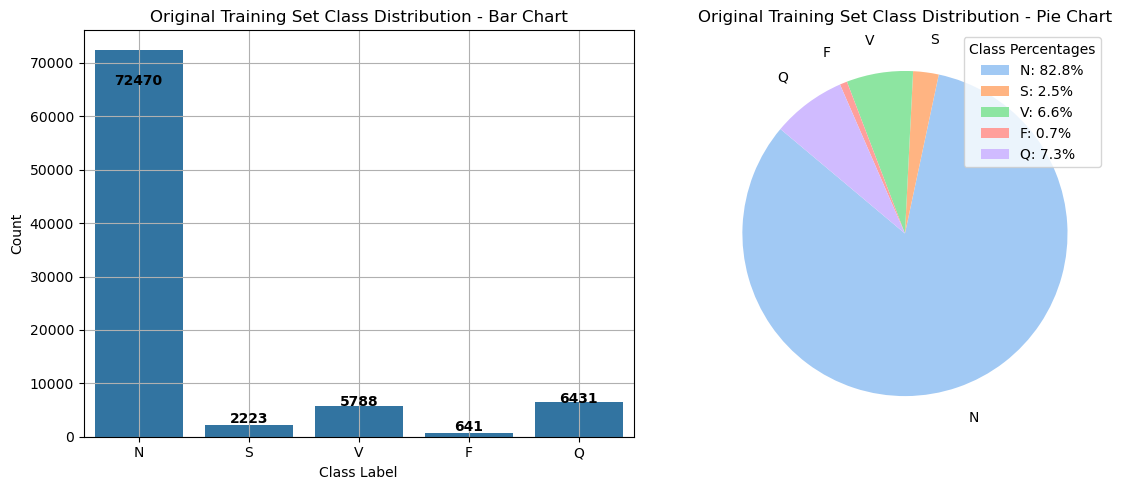
\includegraphics[width=0.5\textwidth]{images/OriginalDatasetTrainingDistribution.png}
    \caption{Original Trainng Dataset Distribution}
    \label{fig:original_trainset_distribution}
\end{figure}

\begin{figure}[htbp]
    \centering
    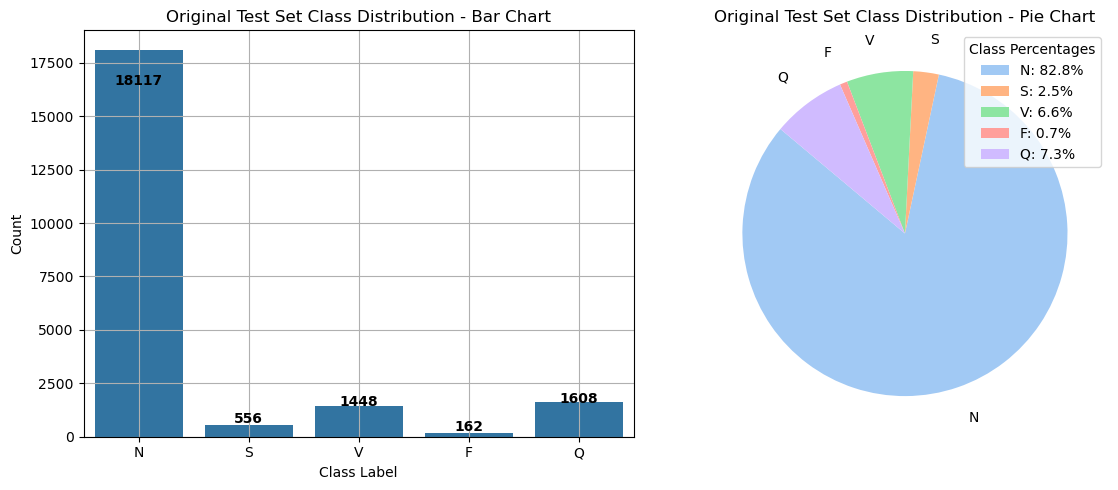
\includegraphics[width=0.5\textwidth]{images/OriginalDatasetTestDistribution.png}
    \caption{Original Test Dataset Distribution}
    \label{fig:original_testset_distribution}
\end{figure}

\begin{figure}[htbp]
    \centering
    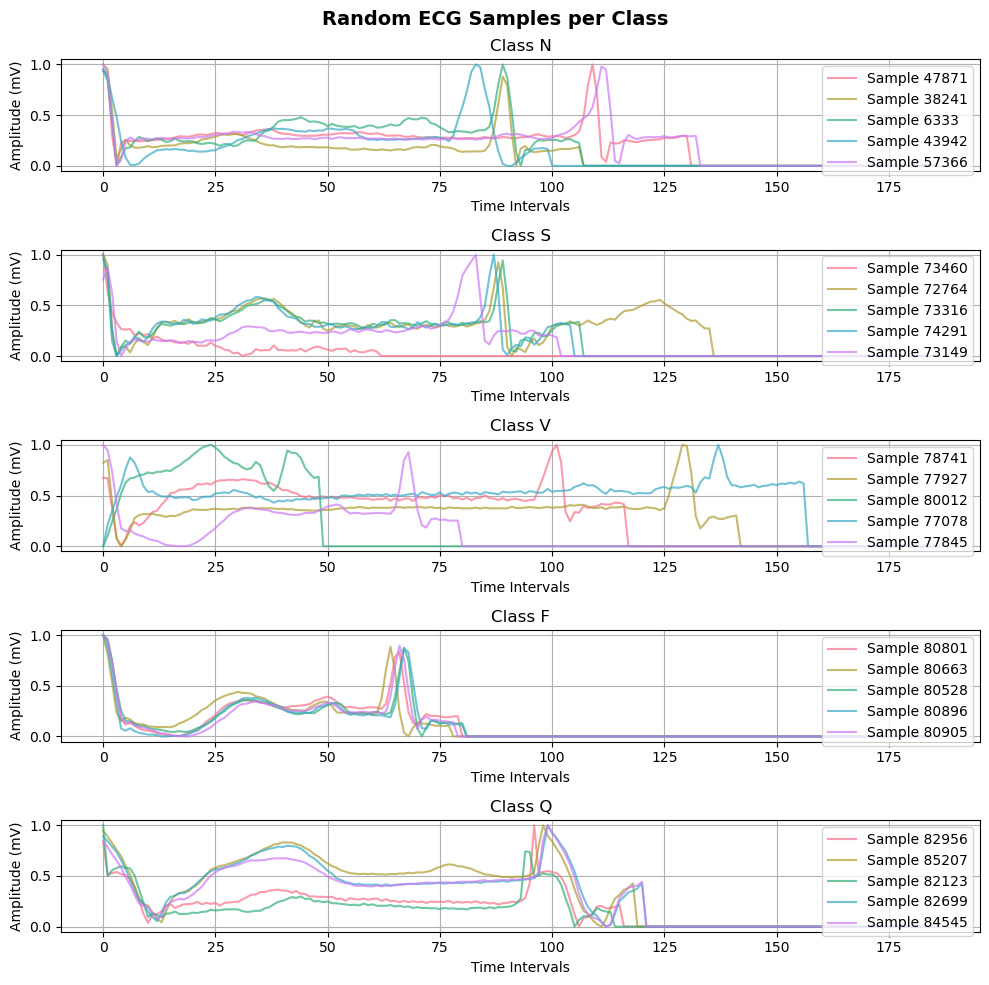
\includegraphics[width=0.5\textwidth]{images/RandomECGsamplesPerClass.png}
    \caption{ECG Heartbeat Samples}
    \label{fig:ecg_samples}
\end{figure}


\section{System Engineering}
In this chapter, the system implementation is described using the flow chart from figure \ref{fig:flowchart}. 

\begin{figure}
    \begin{center}
        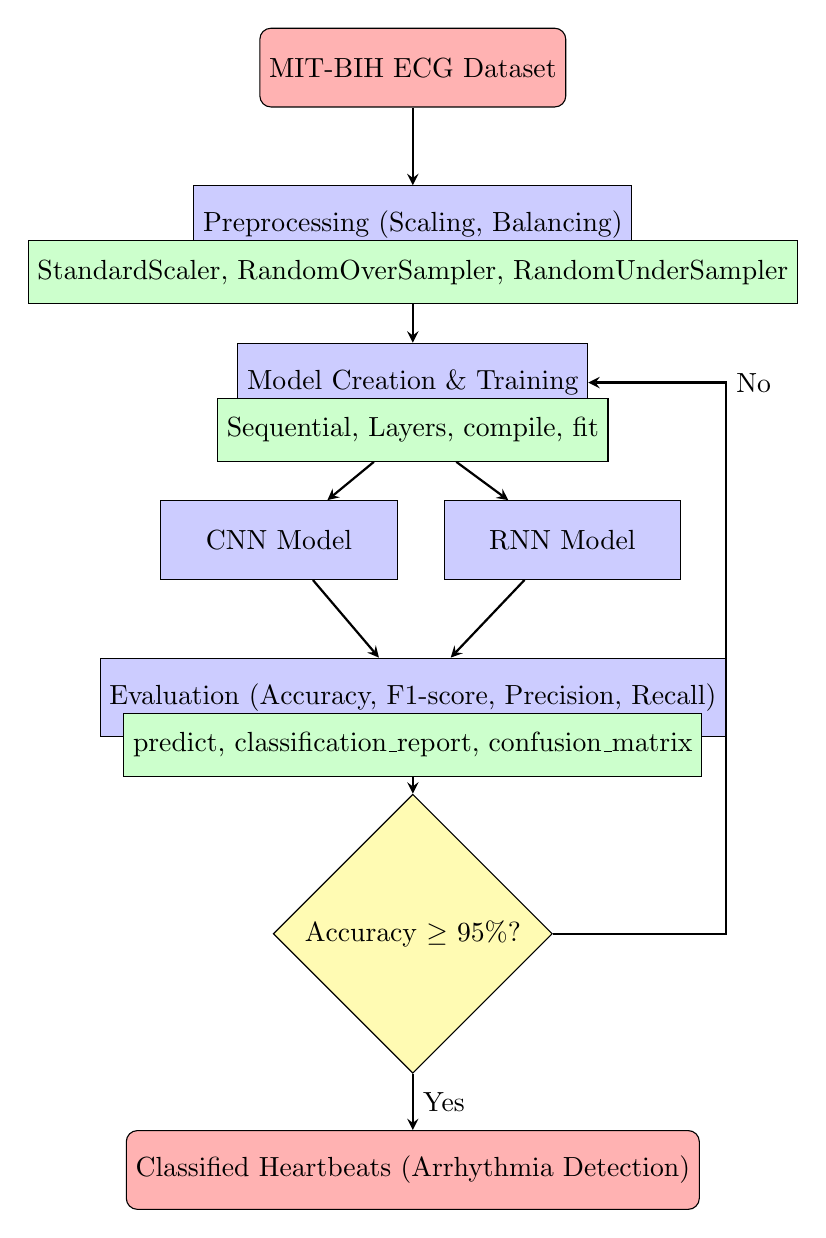
\begin{tikzpicture}[node distance=2cm]
            % Nodes
            \node (input) [startstop] {MIT-BIH ECG Dataset};
            \node (preprocess) [process, below of=input] {Preprocessing (Scaling, Balancing)};
            \node (training) [process, below of=preprocess] {Model Creation \& Training};
            \node (cnn) [process, below of=training, xshift=-1.7cm] {CNN Model};
            \node (rnn) [process, right of=cnn, xshift=1.6cm] {RNN Model};
            %\node (fusion) [process, below of=cnn] {Model Fusion (Ensemble or Best Model)};
            \node (evaluation) [process, below of=cnn, xshift=1.7cm] {Evaluation (Accuracy, F1-score, Precision, Recall)};
            \node (decision) [decision, below of=evaluation, yshift=-1cm] {Accuracy $\geq$ 95\%?};
            \node (output) [startstop, below of=decision, yshift=-1cm] {Classified Heartbeats (Arrhythmia Detection)};
    
            % Commands and data flow
            \node (cmd-preprocess) [command, right of=preprocess, yshift=-0.6cm, xshift=-2cm] {StandardScaler, RandomOverSampler, RandomUnderSampler};
            \node (cmd-training) [command, right of=training, yshift=-0.6cm, xshift=-2cm] {Sequential, Layers, compile, fit};
            \node (cmd-evaluation) [command, right of=evaluation, yshift=-0.6cm, xshift=-2cm] {predict, classification\_report, confusion\_matrix};
            
            % Arrows
            \draw [arrow] (input) -- (preprocess);
            \draw [arrow] (cmd-preprocess) -- (training);
            \draw [arrow] (cmd-training) -- (cnn);
            \draw [arrow] (cmd-training) -- (rnn);
            \draw [arrow] (cnn) -- (evaluation);
            \draw [arrow] (rnn) -- (evaluation);
            \draw [arrow] (cmd-evaluation) -- (decision);
            \draw [arrow] (decision.east) -- ++(2.2,0) |- (training.east) node[midway, right] {No};
            \draw [arrow] (decision) -- (output) node[midway, right] {Yes};
        \end{tikzpicture}
    \end{center}
    \caption{Flowchart of the System}
    \label{fig:flowchart}
\end{figure}
    
The system consists of the following steps: data preprocessing, model training, model evaluation. The data preprocessing step involves loading the dataset, splitting the dataset into training, validation and testing sets. The data of training and validation set are normalized and balanced. To balance the dataset we've decided not to use any synthetic data generation, like the SMOTE (Synthetic Minority Over-sampling Technique) or ADASYN (Adaptive Synthetic Sampling) algorithms to oversample the minority classes, because of the risk that it may create artificial data that does not represent real data. Instead, we've decided to undersample the majority class by 50\% using random undersampling and oversample using random oversampling for the minority classes to balance the dataset. Random oversampling creates new samples by randomly selecting samples from the minority classes and simply duplicates them.
Normalizing the data is done using the StandardScaler from the scikit-learn library.
The balanced dataset distribution is shown in figure \ref{fig:balanced_trainset_distribution}. 

\begin{figure}[htbp]
    \centering
    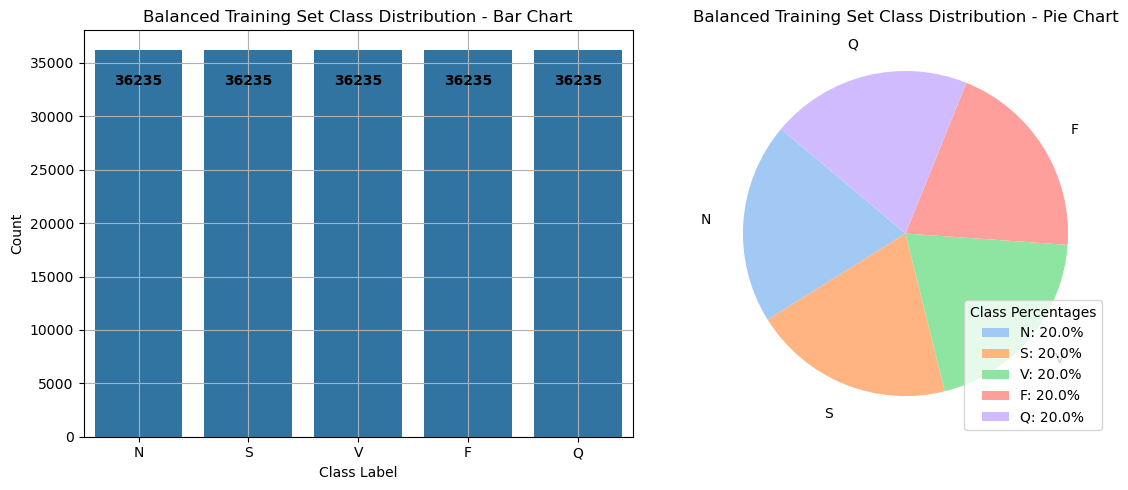
\includegraphics[width=0.5\textwidth]{images/BalancedDatasetTrainingDistribution.png}
    \caption{Balanced Trainng Dataset Distribution}
    \label{fig:balanced_trainset_distribution}
\end{figure}

The model training step involves building the deep learning models, training the models on the training set, validating on a validation set using 80\% to 20\% split, and saving the model. The model evaluation step involves evaluating the model on the test set and calculating the accuracy, precision, recall and f1-score.



\section{Algorithm Design Using Spiral Approach}
The algorithm design for the ECG heartbeat classification system is based on the spiral approach, which involves iterative development and refinement of the system. 

Based on gained knowledge from the course and literature such as in \cite{b3}, \cite{b4} and \cite{b5} on ECG classification two algorithms were chosen to be examined on their performance on ECG heartbeat classification: Convolutional Neural Networks (CNN) and Recurrent Neural Networks (RNNs). CNNs automatically learn and extract relevant features from raw ECG signals, by recognizing characteristic wave patters. Limitations of CNNs are their limitation to a fixed receptive field, they might overlook long-term dependencies in the heartbeat sequence. 
Recurrent neural networks like LSTMs (Long Short-Term Memory) and GRUs (Gated Recurrent Units) are designed to capture temporal dependencies in time-series data such as ECG. LSTMs maintain memory cells with gated updates, allowing them to retain information over extended periods. Notably, they are designed to overcome the vanishing gradient problem in RNNs. GRUs are simplified RNN variant with only update and reset gates, which makes them computationally more efficient than LSTMs.

Combining CNNs with LSTMs or GRU leverages the strengths of both approaches. In these hybrids, the CNN layers first act as feature extractors that convert raw ECG signals into high-level feature sequences, which are then fed into LSTM or GRU layers that model the temporal dynamics. These architectures are effective because they can learn subtle ECG features and also the timing irregularities that signal different arrhythmias. 

\subsection{Model Design for Iteration 1}
The CNN model designed for classification in this project consist of three Convolutional Layers with 32, 64 and 128 filters, kernel size of 3x3, and ReLU activation function. A MaxPooling Layer is used to downsample the feature maps. Before feeding the outputs to a number of Dense Layers a Flatten Layer is used to convert the 2D feature maps to a 1D feature vector. For the Dense layers we use a structure of 64 and 32 neurons with ReLU activation function. The output layer consists of five neurons, one for each class, and uses the softmax activation function.

The CNN-LSTM model consists of a CNN model with three Convolutional Layers and a MaxPooling Layer, and then fed into the LSTM layer. The LSTM layer consists of 64 units. Its output is than flattened and fed into two Dense Layers with 64 and 32 neurons utilizing ReLU activation function. In between the Dense layers a Dropout layer with dropout rate 0.25 is used to prevent overfitting.
The output layer stays the same, it has 5 neurons.

For the CNN-GRU model the same architecture is used, but instead of the LSTM layer a GRU layer with 65 units is used.

The models are trained using the Adam optimizer with a learning rate of 0.001, a batch size of 64, and a categorical cross-entropy loss function. The models are trained for 20 epochs using batch size 32. Callbacks have been used to save the best model based on the validation accuracy and early stopping with a patience of 5 epochs to prevent overfitting and reduce training time. The learning rate is reduced by a factor of 0.5 if the validation loss does not improve for 3 epochs.
The training data is split into 80\% training and 20\% validation data. The model with the best validation accuracy is saved and evaluated on the test dataset.

\subsection{Model Evaluation for Iteration 1}
The models are evaluated based on their performance metrics on the test set. The performance metrics include accuracy, precision, recall, and F1-score. The confusion matrices are used to evaluate the models' performance on each class. The training time of the models is also considered as a performance metric.
In table \ref{tab:model_performance} the performance metrics of the models on the test set are compared. The CNN and CNN-GRU model basically have the same performance, their accuracy, precision, recall, and F1-score are 98.36\%. The CNN-LSTM model has an accuracy of 98.20\%. Looking at the confusion matrices in table \ref{tab:confusion_matrices} and \ref{tab:normalized_conf_percent}, one can see that classes 1 and 3 are the most difficult to classify. The CNN-LSTM model has the best performance on class 1, while the CNN model has the best performance on class 3 classes. The CNN-LSTM model has the wors performance on these difficult classes but performs well on the other classes. From this we can not conclude which model performs best, but the CNN and CNN-GRU model have the same performance and the CNN-LSTM model has a slightly worse performance. Important to note is that the CNN model has the significantly shortest training time of 8minutes, while the CNN-LSTM model has the longest training time of 94 minutes. The CNN-GRU model has a training time of 74 minutes. The CNN model is the most efficient model in terms of training time and performance.

Next we try to improve the performance of the models especially on class 1 and 3 by changing the architecture.

\begin{table}[bt]
    \centering
    \caption{Comparison of Model Performance Metrics (Iteration 1)}
    \label{tab:model_performance}
    \begin{tabular}{lcccccc}
        \toprule
        \textbf{Model} & \textbf{Training Time} & \textbf{Acc.} & \textbf{Prec.} & \textbf{Rec.} & \textbf{F1} \\
        \midrule
        CNN\_It\_1     & 8min 4.4s  & 98.36\% & 98.36\% & 98.36\% & 98.36\% \\
        CNN\_LSTM\_It\_1 & 94min 4.9s & 98.20\% & 98.27\% & 98.20\% & 98.23\% \\
        CNN\_GRU\_It\_1  & 74min 33.7s & 98.36\% & 98.36\% & 98.36\% & 98.36\% \\
        \bottomrule
    \end{tabular}
\end{table}

\begin{table}[ht]
    \centering
    \caption{Comparison of Confusion Matrices for Iteration 1 Models}
    \label{tab:confusion_matrices}
    \begin{minipage}{0.32\textwidth}
        \centering
        \caption*{CNN\_Model\_Iteration\_1}
        \begin{tabular}{cccccc}
            \toprule
            & \multicolumn{5}{c}{Predicted} \\
            \cmidrule(lr){2-6}
            Actual & 0 & 1 & 2 & 3 & 4 \\
            \midrule
            0 & 17957 & 81  & 46  & 17  & 16 \\
            1 & 95    & 453 & 7   & 0   & 1  \\
            2 & 36    & 1   & 1392& 18  & 1  \\
            3 & 13    & 0   & 12  & 137 & 0  \\
            4 & 12    & 1   & 1   & 0   & 1594 \\
            \bottomrule
        \end{tabular}
    \end{minipage}
    \hfill
    \begin{minipage}{0.32\textwidth}
        \centering
        \caption*{CNN\_LSTM\_Model\_Iteration\_1}
        \begin{tabular}{cccccc}
            \toprule
            & \multicolumn{5}{c}{Predicted} \\
            \cmidrule(lr){2-6}
            Actual & 0 & 1 & 2 & 3 & 4 \\
            \midrule
            0 & 17913 & 136 & 32  & 12  & 24 \\
            1 & 74    & 474 & 4   & 3   & 1  \\
            2 & 33    & 5   & 1383& 23  & 4  \\
            3 & 15    & 0   & 12  & 135 & 0  \\
            4 & 13    & 2   & 1   & 0   & 1592 \\
            \bottomrule
        \end{tabular}
    \end{minipage}
    \hfill
    \begin{minipage}{0.32\textwidth}
        \centering
        \caption*{CNN\_GRU\_Model\_Iteration\_1}
        \begin{tabular}{cccccc}
            \toprule
            & \multicolumn{5}{c}{Predicted} \\
            \cmidrule(lr){2-6}
            Actual & 0 & 1 & 2 & 3 & 4 \\
            \midrule
            0 & 17948 & 81  & 40  & 19  & 29 \\
            1 & 77    & 466 & 11  & 0   & 2  \\
            2 & 28    & 6   & 1389& 19  & 6  \\
            3 & 15    & 1   & 17  & 129 & 0  \\
            4 & 7     & 0   & 2   & 0   & 1599 \\
            \bottomrule
        \end{tabular}
    \end{minipage}
\end{table}

\begin{table}[ht]
    \centering
    \caption{Normalized Confusion Matrices in Percent}
    \label{tab:normalized_conf_percent}
    % First Model: CNN_Model_Iteration_1
    \begin{minipage}{0.32\textwidth}
        \centering
        \caption*{CNN\_Model\_Iteration\_1}
        \begin{tabular}{cccccc}
            \toprule
            & \multicolumn{5}{c}{Predicted} \\
            \cmidrule(lr){2-6}
            Actual & 0 & 1 & 2 & 3 & 4 \\
            \midrule
            0 & 99.12\% & 0.45\% & 0.25\% & 0.09\% & 0.09\% \\
            1 & 17.09\% & 81.47\% & 1.26\% & 0.00\% & 0.18\% \\
            2 & 2.49\%  & 0.07\% & 96.13\% & 1.24\% & 0.07\% \\
            3 & 8.02\%  & 0.00\% & 7.41\%  & 84.57\% & 0.00\% \\
            4 & 0.75\%  & 0.06\% & 0.06\%  & 0.00\% & 99.13\% \\
            \bottomrule
        \end{tabular}
    \end{minipage}
    \hfill
    % Second Model: CNN_LSTM_Model_Iteration_1
    \begin{minipage}{0.32\textwidth}
        \centering
        \caption*{CNN\_LSTM\_Model\_Iteration\_1}
        \begin{tabular}{cccccc}
            \toprule
            & \multicolumn{5}{c}{Predicted} \\
            \cmidrule(lr){2-6}
            Actual & 0 & 1 & 2 & 3 & 4 \\
            \midrule
            0 & 98.87\% & 0.75\% & 0.18\% & 0.07\% & 0.13\% \\
            1 & 13.31\% & 85.25\% & 0.72\% & 0.54\% & 0.18\% \\
            2 & 2.28\%  & 0.35\% & 95.51\% & 1.59\% & 0.28\% \\
            3 & 9.26\%  & 0.00\% & 7.41\%  & 83.33\% & 0.00\% \\
            4 & 0.81\%  & 0.12\% & 0.06\%  & 0.00\% & 99.00\% \\
            \bottomrule
        \end{tabular}
    \end{minipage}
    \hfill
    % Third Model: CNN_GRU_Model_Iteration_1
    \begin{minipage}{0.32\textwidth}
        \centering
        \caption*{CNN\_GRU\_Model\_Iteration\_1}
        \begin{tabular}{cccccc}
            \toprule
            & \multicolumn{5}{c}{Predicted} \\
            \cmidrule(lr){2-6}
            Actual & 0 & 1 & 2 & 3 & 4 \\
            \midrule
            0 & 99.07\% & 0.45\% & 0.22\% & 0.10\% & 0.16\% \\
            1 & 13.85\% & 83.81\% & 1.98\% & 0.00\% & 0.36\% \\
            2 & 1.93\%  & 0.41\% & 95.93\% & 1.31\% & 0.41\% \\
            3 & 9.26\%  & 0.62\% & 10.49\% & 79.63\% & 0.00\% \\
            4 & 0.44\%  & 0.00\% & 0.12\% & 0.00\% & 99.44\% \\
            \bottomrule
        \end{tabular}
    \end{minipage}
\end{table}

\subsection{Model Design for Iteration 2}
In the second iteration, the models are improved by adding residual connections to the CNN layers. Residual connections are used to prevent the vanishing gradient problem and allow for deeper networks. The CNN parts of all the models are extended by adding residual connections between the convolutional layers. The models are trained using the same hyperparameters as in the first iteration.

This change did not lead to any improvements, therefor the models are reverted to the original architecture. 

\subsection{Model Design for Iteration 3}
In the third iteration, the models are improved by adding batch normalization layers after each convolutional layer. Batch normalization layers are used to normalize the activations of the previous layer at each batch. This helps to stabilize and speed up the training process. 
For both CNN-LSTM and CNN-GRU models, the LSTM and GRU layers are extended by introducing bidirectional layers. Bidirectional layers process the input sequence in both forward and backward directions, capturing dependencies in both directions. Instead of flattening the entire sequence output from the recurrent layers, global average pooling is used to reduce the sequence to a single vector. The global average pooling computes the average over the time dimension as it often leads to better generalization. An additional dropout layer is added after the last dense layer to prevent overfitting.
The models are trained using the same hyperparameters as in the first iteration.

\subsection{Model Evaluation for Iteration 3}
The performance metrics of the refined models are shown in table \ref{tab:eval_metrics_it3}. The CNN model has an accuracy of 97.88\%, the CNN-LSTM model has an accuracy of 98.20\%, and the CNN-GRU model has an accuracy of 98.04\%. The refined models have not improved the performance. Precision, recall and f1-score are also lower than in the first iteration.

\begin{table}[hbt]
    \centering
    \caption{Performance Metrics for Refined Iteration 3 Models}
    \label{tab:eval_metrics_it3}
    \begin{tabular}{lcccccc}
        \toprule
        \textbf{Model} & \textbf{Training Time} & \textbf{Accuracy} & \textbf{Prec.} & \textbf{Rec.} & \textbf{F1} \\
        \midrule
        CNN\_It\_1     & 8min 4.4s  & 98.36\% & 98.36\% & 98.36\% & 98.36\% \\
        CNN\_LSTM\_It\_1 & 94min 4.9s & 98.20\% & 98.27\% & 98.20\% & 98.23\% \\
        CNN\_GRU\_It\_1  & 74min 33.7s & 98.36\% & 98.36\% & 98.36\% & 98.36\% \\

        CNN\_It\_3      & 34min 33.9s & 97.88\% & 89.01\% & 90.72\% & 89.82\% \\
        CNN\_LSTM\_It\_3 & 28min 20.7s & 98.20\% & 89.67\% & 91.90\% & 90.75\% \\
        CNN\_GRU\_It\_3  & 30min 50.9s & 98.04\% & 87.82\% & 92.90\% & 90.14\% \\
        \bottomrule
    \end{tabular}
\end{table}

The confusion matrices in table \ref{tab:conf_abs_it3} and \ref{tab:conf_matrices_it3} show the models performance on the classification task of the test set. The CNN models correct classification rate on class 1 increased by 1\%, but it missclassifies 6\% more of class 3. The CNN-LSTM models performs slightly worse on all classes. The changes only had a postive effect on the CNN-GRU model, as it has increased its performance on class 3 from before 79.63\% to now 87.04\%. It also does not perform significantly worse on any other class. The training time of the models is between 28 and 34 minutes, with the CNN-LSTM model having the shortest training time.

\begin{table}[ht]
    \centering
    \caption{Confusion Matrices with Absolute Values}
    \label{tab:conf_abs_it3}
    \begin{minipage}{0.32\textwidth}
        %\centering
        \caption*{CNN\_Model\_Iteration\_3}
        \begin{tabular}{cccccc}
            \toprule
            & \multicolumn{5}{c}{Predicted} \\
            \cmidrule(lr){2-6}
            Actual & 0 & 1 & 2 & 3 & 4 \\
            \midrule
            0 & 17864 & 147 & 69  & 10  & 27  \\
            1 & 87    & 459 & 8   & 2   & 0   \\
            2 & 26    & 6   & 1390& 19  & 7   \\
            3 & 16    & 0   & 20  & 126 & 0   \\
            4 & 13    & 5   & 3   & 0   & 1587\\
            \bottomrule
        \end{tabular}
    \end{minipage}
    \hfill
    \begin{minipage}{0.32\textwidth}
        %\centering
        \caption*{CNN\_LSTM\_Model\_Iteration\_3}
        \begin{tabular}{cccccc}
            \toprule
            & \multicolumn{5}{c}{Predicted} \\
            \cmidrule(lr){2-6}
            Actual & 0 & 1 & 2 & 3 & 4 \\
            \midrule
            0 & 17914 & 116 & 44  & 20  & 23  \\
            1 & 85    & 458 & 10  & 3   & 0   \\
            2 & 33    & 3   & 1392& 18  & 2   \\
            3 & 15    & 0   & 13  & 134 & 0   \\
            4 & 6     & 1   & 2   & 1   & 1598\\
            \bottomrule
        \end{tabular}
    \end{minipage}
    \hfill
    \begin{minipage}{0.32\textwidth}
        %\centering
        \caption*{CNN\_GRU\_Model\_Iteration\_3}
        \begin{tabular}{cccccc}
            \toprule
            & \multicolumn{5}{c}{Predicted} \\
            \cmidrule(lr){2-6}
            Actual & 0 & 1 & 2 & 3 & 4 \\
            \midrule
            0 & 17872 & 122 & 65  & 34  & 24  \\
            1 & 76    & 466 & 10  & 2   & 2   \\
            2 & 27    & 6   & 1388& 23  & 4   \\
            3 & 6     & 1   & 14  & 141 & 0   \\
            4 & 9     & 0   & 2   & 3   & 1594\\
            \bottomrule
        \end{tabular}
    \end{minipage}
\end{table}

\vspace{1em}

\begin{table}[ht]
    \centering
    \caption{Normalized Confusion Matrices in Percent}
    \label{tab:conf_matrices_it3}
    % CNN_Model_Iteration_3
    \begin{minipage}{0.32\textwidth}
        %\centering
        \caption*{CNN\_Model\_Iteration\_3}
        \begin{tabular}{cccccc}
            \toprule
            & \multicolumn{5}{c}{Predicted} \\
            \cmidrule(lr){2-6}
            Actual & 0 & 1 & 2 & 3 & 4 \\
            \midrule
            0 & 98.60\% & 0.81\% & 0.38\% & 0.06\% & 0.15\% \\
            1 & 15.65\% & 82.55\% & 1.44\% & 0.36\% & 0.00\% \\
            2 & 1.80\%  & 0.41\% & 95.99\% & 1.31\% & 0.48\% \\
            3 & 9.88\%  & 0.00\% & 12.35\%& 77.78\% & 0.00\% \\
            4 & 0.81\%  & 0.31\% & 1.87\% & 0.00\% & 98.69\% \\
            \bottomrule
        \end{tabular}
    \end{minipage}
    \hfill
    % CNN_LSTM_Model_Iteration_3
    \begin{minipage}{0.32\textwidth}
        %\centering
        \caption*{CNN\_LSTM\_Model\_Iteration\_3}
        \begin{tabular}{cccccc}
            \toprule
            & \multicolumn{5}{c}{Predicted} \\
            \cmidrule(lr){2-6}
            Actual & 0 & 1 & 2 & 3 & 4 \\
            \midrule
            0 & 98.88\% & 0.64\% & 0.24\% & 0.11\% & 0.13\% \\
            1 & 15.29\% & 82.37\% & 1.80\% & 0.54\% & 0.00\% \\
            2 & 2.28\%  & 0.21\% & 96.13\% & 1.24\% & 0.14\% \\
            3 & 9.26\%  & 0.00\% & 8.02\%  & 82.72\% & 0.00\% \\
            4 & 0.37\%  & 0.62\% & 0.12\%  & 0.62\% & 99.38\% \\
            \bottomrule
        \end{tabular}
    \end{minipage}
    \hfill
    % CNN_GRU_Model_Iteration_3
    \begin{minipage}{0.32\textwidth}
        %\centering
        \caption*{CNN\_GRU\_Model\_Iteration\_3}
        \begin{tabular}{cccccc}
            \toprule
            & \multicolumn{5}{c}{Predicted} \\
            \cmidrule(lr){2-6}
            Actual & 0 & 1 & 2 & 3 & 4 \\
            \midrule
            0 & 98.65\% & 0.67\% & 0.36\% & 0.19\% & 0.13\% \\
            1 & 13.67\% & 83.81\% & 1.80\% & 0.36\% & 0.36\% \\
            2 & 1.86\%  & 0.41\% & 95.86\% & 1.59\% & 0.28\% \\
            3 & 3.70\%  & 0.62\% & 8.64\%  & 87.04\% & 0.00\% \\
            4 & 0.56\%  & 0.00\% & 0.12\%  & 0.19\% & 99.13\% \\
            \bottomrule
        \end{tabular}
    \end{minipage}
\end{table}

The problems in classification of classes 1 (Supraventricular) and 3 (Fusion) are still present. The models are not able to classify these classes correctly, probably due to their low number of samples in the used dataset. Also, looking at the random examples of each each classes heartbeats, for the untrained eye the differnces between the classes are not clear. 
The models are not able to learn the features of these classes well enough, so they can not generalize well on these classes, which is a problem for real-world applications. The models are not able to detect these arrhythmias, which can be dangerous for patients. The models need to be improved to be able to classify these classes correctly. 

\section{Consolidation of Performance and Future Plan}
This section consolidates the performance of our ECG classification models and outlines suggestions for future work to enhance model performance and address the limitations observed in the current implementation.

\subsection{Consolidation of Performance}
The overall performance of our ECG classification was evaluated using multiple metrics, including accuracy, precision, recall and F1-score. The models trained in Iteration 1 already had really good performance, the best with an accuracy of 98.76\% with a training time of only 8minutes.
However, a closer look at the per-class performance revealed that certain classes—especially classes 1 and 3 were more challenging. The performance disparities in these classes suggest that while the models are robust overall, the discriminative features for these underperforming classes are not being captured optimally. This could be due to the class imbalance in the dataset, which may have led to the models being biased towards the majority classes. To address this issue, we suggest to experiment with different data augmentation techniques, such as SMOTE, ADASYN instead of simply utilizing Random Oversampling, to balance the dataset and improve the models' performance on the underrepresented classes. 
Moreover, training times were within acceptable limits (ranging from approximately 8 to 100 minutes per model), indicating that the proposed architectures are computationally efficient for the current dataset.

Our ECG classification models were developed and evaluated based on the project specifications metioned in the Requirement and Data Analysis section \ref{sec:project-specs}. The models (CNN, CNN-LSTM, and CNN-GRU) achieved overall accuracies well above the 95\% target and completed training in under 100 minutes, far below the five hour limit. However, while the overall metrics are satisfactory, the per-class performance, especially for arrhythmia classes, suggests room for improvement in recall and precision.

Table~\ref{tab:current_specs} below summarizes the current specifications alongside our achieved results and comments for further improvement:

\begin{table}[b]
    \centering
    \caption{Current Project Specifications vs. Achieved Performance}
    \label{tab:current_specs}
    \begin{tabular}{|p{4.2cm}|p{4.0cm}|p{1.7cm}|p{5.2cm}|}
        \hline
        \textbf{Specification} & \textbf{Requirement} & \textbf{Met?} & \textbf{Comments / Actions} \\
        \hline
        Dataset & MIT-BIH Arrhythmia (5 classes) & Yes & Standard dataset used as specified. \\
        \hline
        Overall Accuracy & $\geq$95\% on test dataset & Yes & All models exceed 95\% (e.g., CNN: 98.36\%). \\
        \hline
        Training Time & $\leq$ 5 hours on M2 MacBook Air & Yes & Training times are within 8-95 minutes. \\
        \hline
        Generalization & Robust performance on unseen ECG signals & Partially & Some overfitting observed; further validation on external data is needed. \\
        \hline
        Performance Metrics & Evaluate using accuracy, precision, recall, F1-score & Yes & Overall metrics are reported; however, per-class performance needs enhancement. \\
        \hline
    \end{tabular}
\end{table}

\subsection{Future Work}
Based on our evaluation, we propose additional specifications for future work to address the shortcomings and further improve model performance:

\begin{enumerate}
    \item \textbf{Per-Class Recall Target:} Increase the recall (sensitivity) for clinically critical arrhythmia classes to at least 90\%.
    \item \textbf{Per-Class Precision Target:} Improve the precision for arrhythmia classes (especially classes 1 and 3) to a target of 90\% or higher.
    \item \textbf{Robust Generalization:} Validate model performance on additional external ECG datasets to ensure robustness across different populations and recording conditions.
\end{enumerate}

By setting additional targets for per-class performance, future iterations should aim to not only meet but exceed the clinical requirements for reliable and robust ECG classification.


\section{Conclusion}
The project aimed to develop a deep learning model for ECG heartbeat classification using the MIT-BIH Arrhythmia Dataset. The model classifies ECG heartbeats into five distinct categories while achieving a minimum accuracy of 95\% on the test dataset. Various AI models were compared and evaluated based on key performance metrics, including accuracy, precision, recall, and F1-score. Furthermore the model was required to generalize well, avoid overfitting and ensure robustness on unseen ECG signals. The models did generally perform well on the test dataset, but had problems in classifying the Supraventricular and Fusion classes. For real world applications, improvements are needed to ensure reliable classification of these classes and that deseases are not missed.
The models were trained on an M2 MacBook Air within five hours and complied with EU regulations regarding medical AI and GDPR.

\bibliographystyle{IEEEtran}
\bibliography{Insert your bibliography file here}

\begin{thebibliography}{00}
    %\bibitem{citekey} Author(s), “Title of the Paper,” Journal Name, vol. xx, no. xx, pp. xxx-xxx, Month Year.
    \bibitem{b1} Shayan Fazeli, "ECG Heartbeat Categorization Dataset."  https://www.kaggle.com/datasets/shayanfazeli/heartbeat (accessed Mar. 11, 2025).

    \bibitem{b2} “Regulation - EU - 2024/1689 - EN - EUR-LEX.” https://eur-lex.europa.eu/legal-content/EN/TXT/?uri=CELEX\%3A32024R1689 (accessed Mar. 11, 2025).

    \bibitem{b3} S. Raghav and A. K. Mishra, "Fractal feature based ECG arrhythmia classification," TENCON 2008 - 2008 IEEE Region 10 Conference, Hyderabad, India, 2008, pp. 1-5, doi: 10.1109/TENCON.2008.4766475. keywords: {Fractals;Electrocardiography;Databases;Heart rate variability;Frequency;Testing;Classification algorithms;Pattern recognition;Heart beat;Signal processing algorithms;Beat classification;ECG arrhythmia;Fractal dimension},

    \bibitem{b4} Youhe Huang and Hongru Li and Xia Yu, "A novel time representation input based on deep learning for ECG classification," Biomedical Signal Processing and Control, vol. 83, p. 104628, 2023, doi: https://doi.org/10.1016/j.bspc.2023.104628. keywords: {Heartbeat classification, Time characteristic representation, Information Fusion, Deep learning}

    \bibitem{b5} Y. Ansari, O. Mourad, K. Qaraqe, and E. Serpedin, “Deep Learning for ECG Arrhythmia Detection and Classification: An Overview of Progress for Period 2017–2023,” Frontiers in Physiology, vol. 14, doi: 10.3389/fphys.2023.1246746.
\end{thebibliography}

\end{document}